\documentclass[a4paper, 12pt]{report}
\usepackage{ctable}
\usepackage{url}
\usepackage{graphicx}
\usepackage{amsmath}
\usepackage{eurosym}

\title{Software Engineering Group 2 (2009-2010) \\Software Project Management Plan}
\author{Nick De Cooman}
\date {December 13, 2009}

\begin{document}
	
	\maketitle
	
	\setcounter{tocdepth}{1}	
	\tableofcontents
	
	\chapter{Introduction}
	
		\section{Project overview}
		
			The goal of this project is to design and implement the software 
			behind an online auction website such as eBay. The codename of our project 
			is {\emph Salesmen}. 

			This project is embedded in the Software Engineering course, 
			which is designed for senior students of Computer Science and Engineering 
			at the Vrije Universiteit Brussel. It has a threefold purpose:
			
			\begin{enumerate}
				\item Get familiar with the software development process and learn to work
				in a team.
				
				\item Develop a system that supports the functionality of an auction website. 
				This means that a user will be able to sell or buy items in an online auction. 
				
				\item Develop and maintain a general website on our project. Up to date 
				versions of all documents such as minutes, timesheets and deliverables will be 
				available at any time. This site will be hosted at
				\url{http://wilma.vub.ac.be/~se2_0910/}.
			\end{enumerate}	
			
			The software of the application will be written in Java and 
			distributed under an Open Source license.	
		
		\section{Project deliverables}
		
		\begin{itemize}
			
			\item Software documentation (see \ref{deadlines})
			\item Minutes: 3 days after meeting
			\item Timesheets: every Monday before 12H00
			\item Source code
			
		\end{itemize}	
		
		All of those documents will be available in English on our website.
	
		
		\section{Reference materials}
		
			\begin{itemize}
			
				\item 
					\url{http://tinf2.vub.ac.be/~dvermeir/courses/software_engineering/slides.pdf}
			
				\item Eric J. Braude, \emph{Software Engineering -
				An Object-Oriented Perspective}, John Wiley \& Sons, 2001. ISBN 0-471-32208-3.
			
			\end{itemize}
			
		\section{Definitions and acronyms}

			\begin{tabular}{l l}

				\textbf{SCMP} & Software Configuration Management Plan \\
				\textbf{SDD} & Software Design Plan \\
				\textbf{SPMP} & Software Project Management Plan \\
				\textbf{SQAP} & Software Quality Assurance Plan \\
				\textbf{SRS} & Software Requirements Specification \\
				\textbf{STD} & Software Test Document \\
				\textbf{COCOMO} & Constructive Cost Model

			\end{tabular}				
		
		\section{Revision history}
		
			\begin{tabular}{l l l l}
				\\
				\FL Version & Date & Name & Description
				\ML 0.10 & 21/10/09 & Nick De Cooman & Initial draft
				\NN 0.11 & 22/10/09 & Nick De Cooman & Revision after quality control
				\NN 0.20 & 12/11/09 & Nick De Cooman & Revision including customer's comments
				\NN 0.21 & 20/11/09 & Nick De Cooman & Adding estimation of effort
				\NN 0.22 & 22/11/09 & Nick De Cooman & 	- Revision on process model 
				\NN & & &								- Adding real costs
				\NN 0.23 & 23/11/09 & Nick De Cooman & 	Adding Gantt chart 
				\NN 0.24 & 26/11/09 & Nick De Cooman & 	Adding estimation of costs
				\NN 0.30 & 10/12/09 & Nick De Cooman & 	Updating monitoring mechanisms
				\NN 0.31 & 12/12/09 & Nick De Cooman &	- Updating costs
				\NN & &	 &								- Updating Gantt chart
				\\
			\end{tabular}	
		
		
		
	\chapter{Project Organization}
	
		\section{Process model}
		
		The chosen proces model will be the spiral model, with 2 iterations. Unlike
		the waterfall process, we will be able to show partial versions to the customer 
		for feedback, reducing risks such as faulty requirements. The application will 
		consists of some basic functionality after the first iteration and more advanced features will be implemented 
		during the second one. \\
		\\
		A detailed planning of this process can be found in section \ref{planning}.
			
		
		\section{Organizational structure}
		\label{sec:struc}
		
		The structure of our team will be organised as followed:
		
		\subsection{Project Manager}
			\begin{itemize}
				\item Head of the project team
				\item Deliver the SPMP
				\item Risk Analysis
				\item Keep track of the project's progress
				\item Manage timesheets
				\item Prepare and chair meetings
				\item Spokesman to organizational boundaries and interfaces
				\item Motivate and improve internal collaboration
			\end{itemize}
			
		\subsection{Project Secretary}
			\begin{itemize}
				\item Resume meetings
				\item Deliver minutes
			\end{itemize}
			
		\subsection{Configuration Manager}
			\begin{itemize}
				\item Deliver the SCMP
				\item Manage revision control system
				\item Install and maintain used tools
				\item Make backups of all project documents
			\end{itemize}
			
		\subsection{Quality Assurance Manager}
			\begin{itemize}
					\item Head of quality team
					\item Deliver SQAP and STD
					\item Design and implement test framework
					\item Coordinate testing as defined in STD
					\item Verify the general quality of the product
					\item Verify the quality of documents
			\end{itemize}
			
		\subsection{Requirements Manager}
			\begin{itemize}
				\item Deliver SRS
				\item Check whether the requirements are implemented
				\item Look for extra functional requirements
				\item Interview customer related to the requirements
				\item Present final requirements to the customer
			\end{itemize}
			
		\subsection{Design Manager}	
			\begin{itemize}
				\item Head of design team
				\item Deliver SDD based on the SRS
				\item Manage design of the system
				\item Check whether implementation is based on the SDD
				\item Design and manage database according to SRS and SQAP
				\item Present design to the customer
			\end{itemize}	
			
		\subsection{Implementation Manager}
			\begin{itemize}
				\item Head of implementation management
				\item Manage the integration of different parts of the code
				\item Track errors
				\item Define implementation proces based on the SDD	
				\item Manage documentation of code
			\end{itemize}
			
		\subsection{Webmaster}
			\begin{itemize}
				\item Develop and maintain project website
				\item Upload documents, after approval of the project manager
			\end{itemize}	
		
		\section{Organizational boundaries and interfaces}
		
		The external communication with the customer will only happen via the project
		manager, the requirements manager and the design manager. The project manager reports
		major problems, progress status and other organisatorial issues. 
		The requirements manager discusses the functionality of the system and 
		the design manager will present the design of the system to the
		customer.  
		
		\section{Project responsibilities}
		
			The responsibilities, as defined in \ref{sec:struc}, will be 
			associated to the following persons:
		
			\begin{tabular}{l l l}
				\\
				\FL Role & Effective & Assistant
				\ML Project Manager & Nick & Patrick
				\NN Project Secretary & Jonathan & Wouter
				\NN Configuration Manager & Jorne & Sina
				\NN Quality Assurance Manager & Patrick & Bart
				\NN Requirements Manager & Wouter & Jonathan
				\NN Design Manager & Bart & Nick
				\NN Implementation Manager & Sina & Jorne
				\NN Webmaster & Sina & Wouter \\
				\\
			\end{tabular}
			\\
			However, this does not mean that a person is only responsible
			for his/her own function. Every team member can be asked for assistance in all 
			processes in function to achieve the end goal.
			
			A person responsible for creating a deliverable also needs to be aware
			of the fact that
			
			\begin{itemize}
				
				\item Documents will be writen in \LaTeX-format, using the provided template.
				
				\item Documents need to be ready in time (as defined in \ref{deadlines}), and
				sent to the project manager for approval. 
				
				\item Documents needs to be up-to-date during the entire project. 
				
			\end{itemize}
			
	\chapter{Managerial process}
		
		\section{Objectives and priorities}
			
			During the development of the system, the following objectives should be kept
			in mind:
			
			\begin{enumerate}
				
				\item The project should meet the requirements of the customer
				\item Deadlines have to be respected
				\item Reusability and extensibility of the software is very important
				\item The system should be stable
				
			\end{enumerate}	
			
		\section{Assumptions, dependencies and constraints}
			
			\begin{itemize}
				
				\item No assumptions will be made.
				
				\item Dependencies \\
 					  For the project to succeed, it will depend on
					  the knowledge and the motivation of the team members	
				
				\item Constraints:
				\begin{itemize}
					\item Only open-source software is to be used
					\item The product should run in a Linux environment
					\item The product should run on the Wilma server
				\end{itemize}
				
			\end{itemize}	
			
		\section{Risk Management}
			
			Developing software introduces a lot of risks. At regular times these risks will
			be discussed in order to reduce or eliminate them. Each member is encouraged to report
			possible risk to the project leader.
			
			\subsection{Google goes down for a certain period}
			\textbf{Criticality}: + \\
			We need to make daily backups of our files and documentation. This will be 
			performed by the configuration team.
			
			
			\subsection{Lack of knowledge of certain tools or mechanisms}
			\textbf{Criticality}: ++++ \\
			Some tools and mechanisms will be completely new to some team members which can
			results in a lack of knowledge and inefficiency. To prevent this, tutorials will be
			made as Wiki-pages. Moreover, presentations can be given if the subject is 
			too complex or if it demands a complete explanation. 
			
			\subsection{Somebody becomes ill}
			\textbf{Criticality}: +++ \\
			This risk has already been considered in the beginning of this 
			project. This is why there is an Assistant(formerly called Backup) for 
			every Management position. If a leader or manager gets ill, the assistant 
			of that function should be able to fully understand his 
			function and replace that leader or manager, for a certain period of time.
			
			\subsection{Risk Table}
			The above risks can be ranked in a table based on the likelihood of the risks, the
			impact on the project, the cost of disposal and the priority of it. 
			This last one will be calculated as follows :
			\begin{center}
			$ priority = (11 - change) \cdot (11 - effect) \cdot disposal $
			\end{center}
			The lower the priority, the most impact it has on the project. 
			
			\begin{table}
				\begin{center}
			\begin{tabular}{l c c c c}
				\\
				\FL Risk & Change & Effect & Disposal & \textbf{Priority}
				\ML Google down  & 2 & 8 & 8 & \textbf{216}
				\NN Lack of knowledge & 6 & 8 & 6 & \textbf{90}
				\NN Illness & 6 & 4 & 3 & \textbf{105}
			\end{tabular}
			\end{center}
			\caption{Risk table}
			\end{table}
			  
			

		\section{Monitoring and controlling mechanisms}	
			
			\subsection{Meetings}
			Meetings will be held every week. The topics to handle at the meeting will be defined
			in an agenda and will be sent to every team member before the start of the
			meeting. Minutes will summarize the meetings and will be available on the project 
			website within 3 days after the meeting.
			
			Should one not be able to attend the meeting, he/she is requested to inform
			the project manager within 3 hours before the start of the meeting.
			
			\subsection{Timesheets}
			A global timesheet will be available every Monday before 12H00. Team 
			members will need to submit their timesheet on Sunday before 23h59
			for approval by the team manager.
			
			\subsection{SCRUM Report}
			Every 2 weeks all team members should deliver a SCRUM report in which they have to
			answer briefly 3 questions:
			
			\begin{enumerate}
				\item What have you done in the last 2 weeks?
				\item What will you do in the next 2 weeks?
				\item Is there anything preventing you from doing what you have
				planned?
			\end{enumerate}	
			
			In this way, the project manager is able to monitor the global progress of the project
			and directing certain members where necessary. A summarized version will be available
			onto the website afterwards. 
			
			
	\chapter{Technical Process}
	
			\section{Methods, tools and techniques}
			
			\begin{itemize}
				
				\item Google Code \\
				There has been chosen for Google Code because it has some 
				handy features:
				
				\begin{itemize}
			 		\item Revision control system: Subversion in our case, see below.
					\item Issue tracker
					\item Wiki (is sometimes handy e.g. for meeting agenda).
					\item File download server (for our software and document releases).
				\end{itemize}

				\item Subversion \\
				This is a centralized version control system chosen for the 
				following reasons:
				
				\begin{itemize}
					\item It is easy to refactor the source code structure, 
					while preserving files' history.
					\item The whole repository has a single revision that is 
					incremented after each commit.
				\end{itemize}

				\item Eclipse \\
				Eclipse is a software development environment comprising an IDE and 
				a plug-in system to extend it. It is used to develop applications in 
				Java. It was decided to work with Eclipse because 
				it has a very userfriendly interface and because of its popularity. Also it's 
				known by most of the team members.
				
				\item \LaTeX \\
				 \LaTeX{} has been chosen to document this project because it's 
				internationally known and commonly used. Also, a few members 
				were interested in learning this language.
				
			\end{itemize}	
			
			More specific tools will be discussed later.
			
			\section{Software documentation}
			
			Several documents will be publised during the execution of this project. \\
			
			\label{deadlines}
				\begin{tabular}{l l}

					\FL Document & First version available on
					\ML SPMP & October 26, 2009
					\NN SCMP & November 9, 2009
					\NN SRS & November 13, 2009
					\NN SQAP & November 23, 2009
					\NN SDD & November 30, 2009
					\NN STD & December 07, 2009
				\end{tabular}
			
			\section{Project support functions}
			
			Throughout the entire project, Joeri De Koster and Dirk Vermeir will 
			be available for any help. For Wilma related problems, Dirk Van Deun 
			can be contacted.
	
	\chapter{Work packages, schedule and budget}
			
			\section{Costs}
			
			\subsection{Man-costs up to now}
			
			Using timesheets enables us to track the real costs of this project. Off course,
			this only includes man-costs and it does not cover some hidden problems that can occur during
			the development.
			
			Considering the starter wage of a computer scientist is approximately \euro 2200 gross, we can calculate a 
			realistic earning per hour. Assume one should perform an average of 38 hours per week, 
			and a month consists of 4 weeks. This results in:
			\[ \textrm{Wage/hour} = \frac{\textrm{\euro} 2200 \textrm{ wage/month}}{38 \textrm{ hours/week} \cdot 4 \textrm{ weeks/month}} \approx \textrm{\euro} 14,50 \]
			 
			
			In that case, the total cost of this project so far is given in table \ref{realcosts}.
			
			
			\begin{table}
				\begin{center}
			\begin{tabular}{l l l}
				\FL Week & Total hours & Total Cost
				\ML Week 42 & 43 hours & \euro623,50 
				\NN Week 43 & 63 hours & \euro913,50
				\NN Week 44 & 36 hours & \euro522,00
				\NN Week 45 & 60 hours & \euro870,00
				\NN Week 46 & 28 hours & \euro406,00 
				\NN Week 47 & 53 hours & \euro768,50 
				\NN Week 48 & 67 hours & \euro971,50 
				\NN Week 49 & 67 hours & \euro971,50
				\ML \textbf{TOTAL} & \textbf{417 hours} & \textbf{\euro6046,50} 
				\LL
			\end{tabular}
				\end{center}
				\caption{Real costs up to now based on timesheets}
				\label{realcosts}
			\end{table}
			
			\subsection{Estimation of total man-costs}
			
			Based on the information in table \ref{realcosts}, we can estimate the total cost of this project
			by calculating the average number of hours up to now. For the first 8 weeks, the average number of worked hours is \emph{52,1 hours/week}.\\
			
			Assuming 27 weeks will be needed to accomplish this project, the total number of man-hours can be estimated as:
			\[ 52,1 \textrm{ hours/week} \cdot  27 \textrm{ week} \approx 1407 \textrm{ man-hours} \]
			
			Thus, the total man-cost results in:
			\[ 1407 \textrm{ man-hours} \cdot  14,50 \textrm{ euro/hour} = \textrm{\euro} 20.401 \]

			Note that this is just an estimation, and propably amount to \euro 25.000. 
			
			
			
			\subsection{Estimation of effort}
			
			To calculate an estimation of costs, the COCOMO algorithm developed by Barry Boehm
			will be used. Depending on the number of lines of code, the costs and efforts of this
			project can be computed. Off course, this is just an estimation and will differ from
			reality. The algorithm provides next formulas in order to calculate the effort and
			cost:
			
			\begin{center}
			Effort Applied: $ E = a \cdot (KLOC)^{b} $ \\
			Development Time: $ D = c \cdot E^{d} $ \\
			People required: $ P = \frac{E}{D} $ \\
			\end{center}
			
			KLOC is the estimation of the code length expressed in thousands of lines of code.
			Our project can be classified as a semi-detached project which means that our team of
			a medium size has a mixed experience working with a mix of rigid and less than rigid
			requirements. Therefore, the parameters a, b, c, d are defined as in table \ref{par}. 		
			
			
			\begin{table}
				\begin{center}
			\begin{tabular}{l l}
				\FL Parameter & Value
				\ML a & 3.0
				\NN b & 1.12
				\NN c & 2.5
				\NN d & 0.35
			\end{tabular}
				\end{center}
				\caption{COCOMO Parameters for a semi-detached project}
				\label{par}
			\end{table}	
			
			By analyzing simular projects, we estimate to write 10KLOC. This brings the total
			effort to:
			
			\begin{center}
				$ E = 3.0 \cdot 10^{1.12} \approx 39,55 $ man-months
			\end{center}
			
			The total development time thus becomes:
			
			\begin{center}
				$ D = 2,5 \cdot 39,55^{0,35} \approx 9,06 $ months
			\end{center}
			
			This results in a total staff estimation of
			
				\[ P = \frac{39,55 \textrm{ man-months}}{9,06 \textrm{ months}} \approx 4,37 \textrm{ people} \]
			
			Using the COCOMO algorithm, we can thus conclude that 4,37 people are needed to
			realise our project in 9,06 months. 
			
			\section {Dependencies}
			
			At this time, it is only possible to provide 1 general dependency :
			
			\begin{itemize}
				
				\item Iteration 2 depends on the completion of iteration 1.
				
			\end{itemize}
			
			
			\section{Planning}	
				\label{planning}
			\begin{figure}
				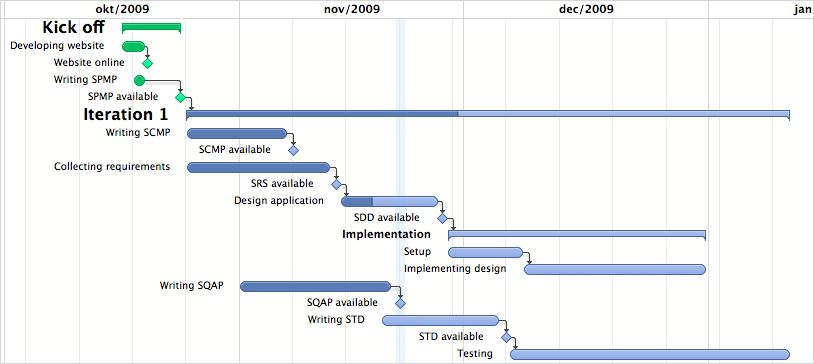
\includegraphics[angle=90, height=20cm]{../../img/gantt-chart.jpg}
				\caption{Current schedule of planning in form of Gantt-chart}
			\end{figure}	
\end{document}
